% MX17 Paper I -- detector & performance. Outline stage.
% Journal and author list undecided (PAPER_PLAN C4): plain article for now; switch
% the class (elsarticle for NIM A, jinst for JINST) once chosen.
\documentclass[11pt,a4paper]{article}
\usepackage[margin=2.2cm,marginparwidth=2.6cm]{geometry}
\usepackage[T1]{fontenc}
\usepackage{lmodern}
\usepackage{amsmath,amssymb}
\usepackage{graphicx}
\usepackage{booktabs}
\usepackage{siunitx}
\usepackage{authblk}
\usepackage[hidelinks]{hyperref}
\usepackage{cleveref}
\usepackage{drafting}
% \draftnotesfalse   % uncomment for a clean read without notes

\graphicspath{{figures/}}

\title{The MX17 resistive-strip Micromegas micro-TPCs: design, operation and performance on cosmic rays and in the SPS H4 beam}
\author{\tbw{author list -- undecided (C4)}}
\date{Outline draft, \today}

\begin{document}
\maketitle

\begin{abstract}
\tbw{Abstract written last. Key numbers: X/Y charge balance 0.49/0.53; no dead time after a spark;
intrinsic resolution 176~\textmu m ($0.30\times$ pitch) in the SPS beam; cosmic angular resolution
\requote{1.15--2.51\textdegree} with the waveform reconstruction of the companion paper.}
\end{abstract}

\ifdraftnotes
\listoftodos[Open items]
\clearpage
\fi

\section{Introduction}\label{sec:intro}
\sectionstate{open}{the X17 programme at n\_TOF (INTC proposal); \texttt{mpgd26} physics-case figures}
\intent{Why a micro-TPC: the X17 search at n\_TOF needs the $e^+e^-$ opening angle, so each chamber must give a
3D track segment from one drift gap. Why resistive strips (spark protection at the n\_TOF flash). What this paper
covers (design, operation, gas, timing, efficiency, resolution on cosmics and in the SPS beam) and what the
companion paper~\cite{paperII} covers (the reconstruction).}

\tbw{Two or three paragraphs. Cite the ATOMKI anomaly~\cite{Krasznahorkay2016}, the $^3$He(n,$e^+e^-$) calculation~\cite{Viviani2022},
Micromegas~\cite{Giomataris1996} and resistive Micromegas~\cite{Alexopoulos2011}.}

\begin{figure}[t]
  \centering
  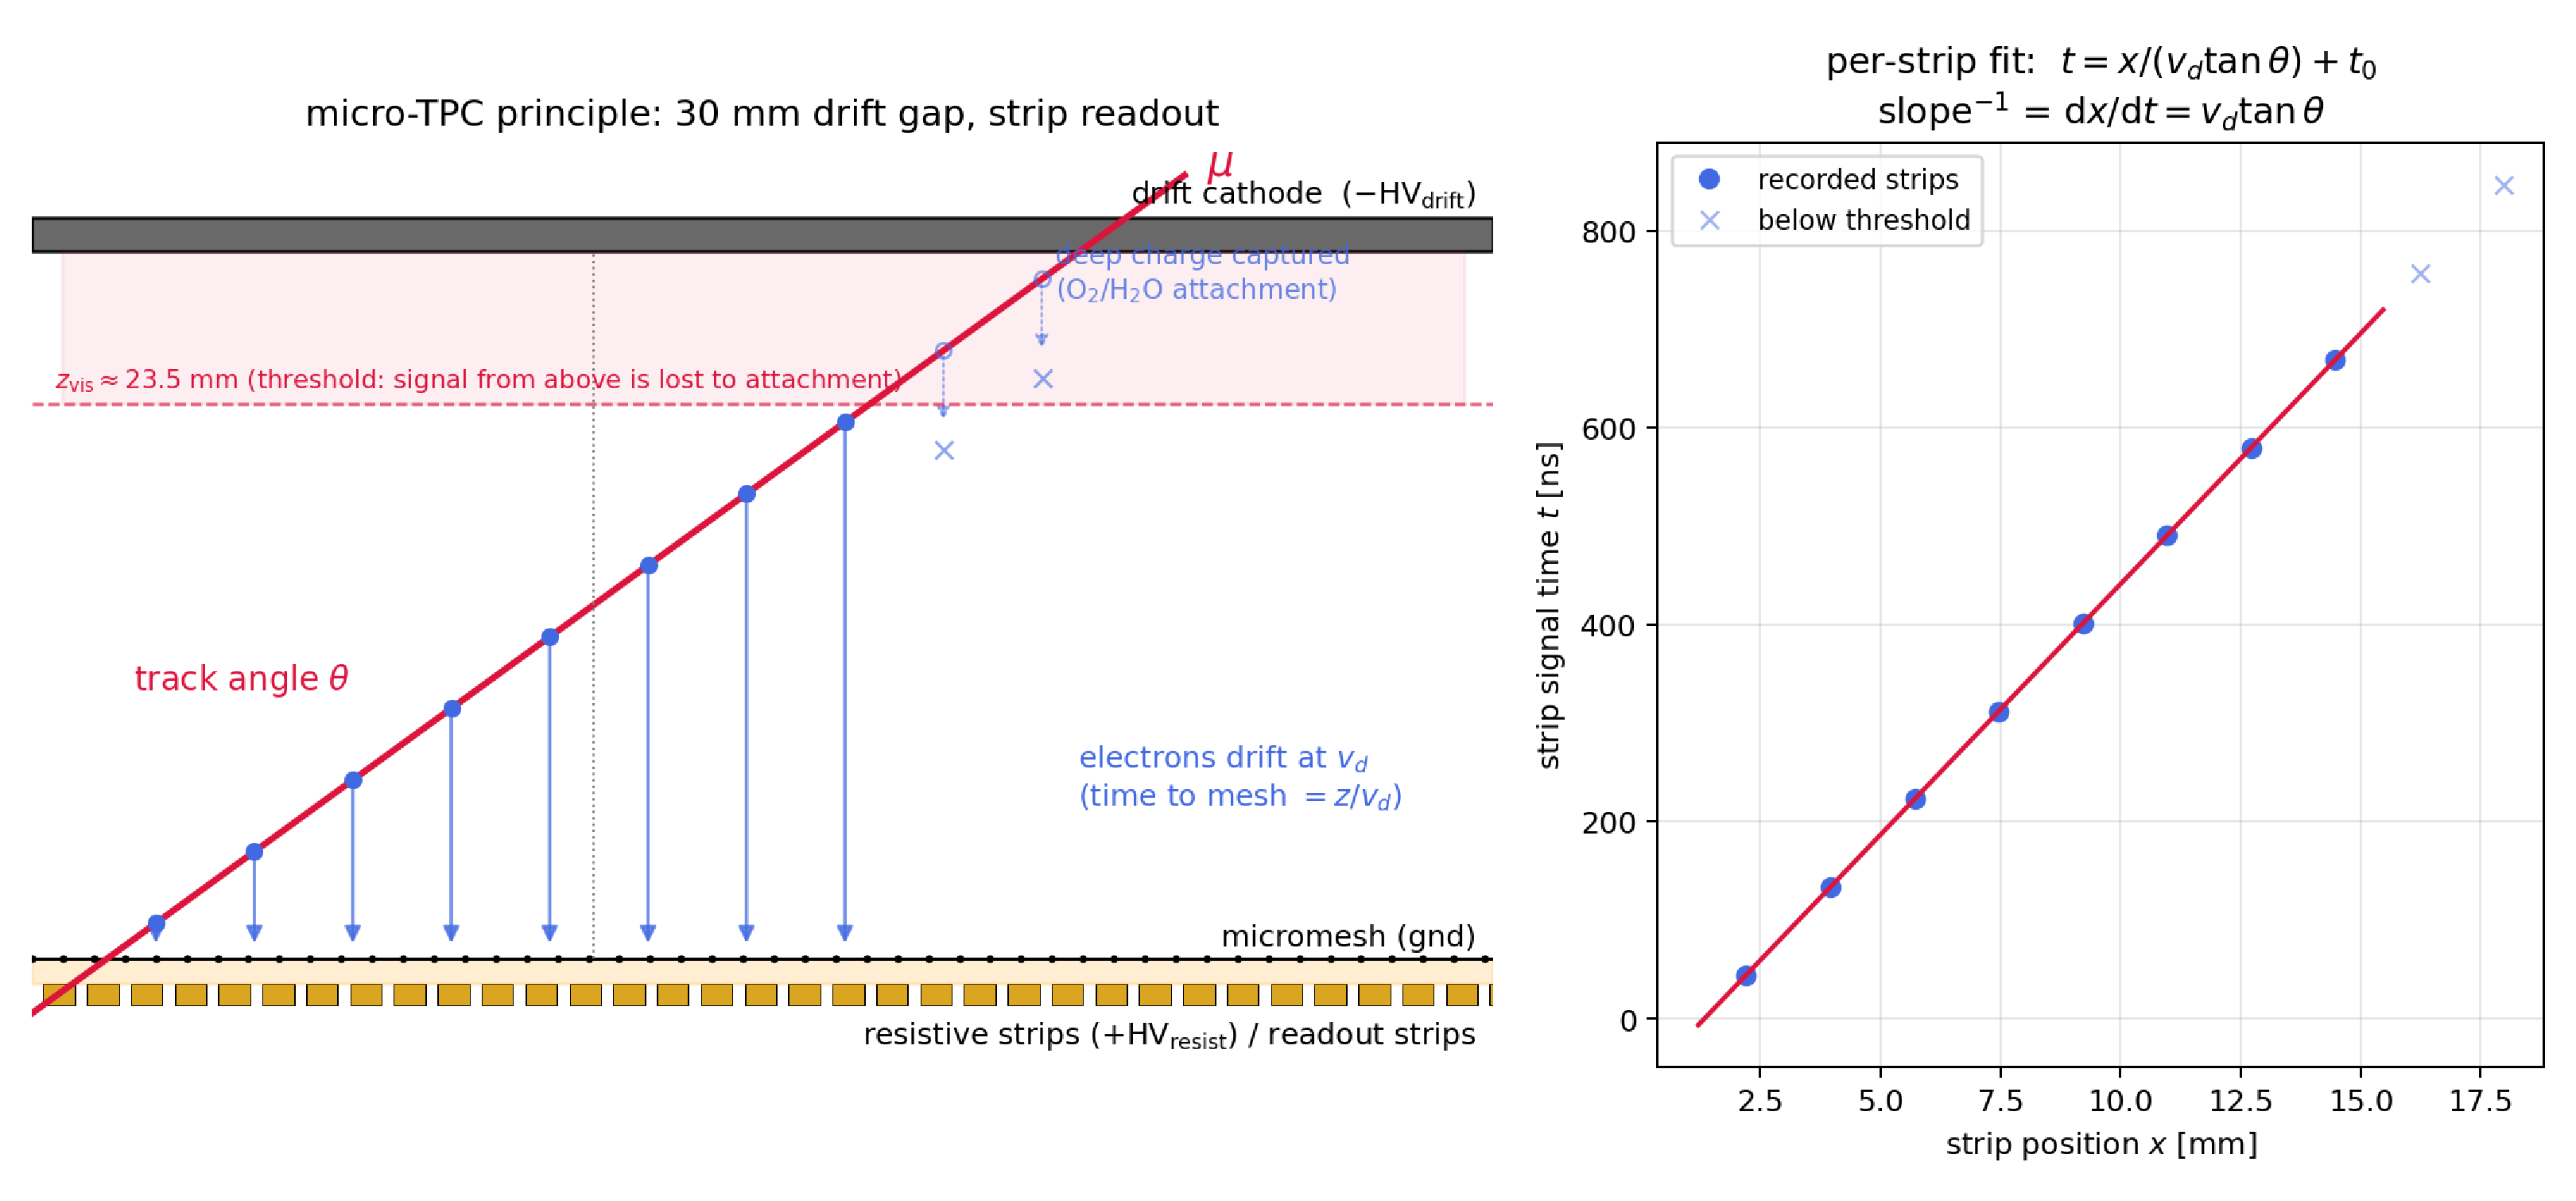
\includegraphics[width=0.85\linewidth]{microtpc_principle}
  \caption{Micro-TPC operation: each strip records the arrival time of its drift electrons, so one 30\,mm gap gives a 3D track segment.}
  \label{fig:microtpc}
\end{figure}

\section{Design and construction}\label{sec:design}
\sectionstate{partial}{\texttt{docs/detector\_spec/spec.py} (97 numbers, 9 unknown, 31 assumed);
spec page \texttt{notes/mx17-detector-spec.html}; Gerber files; PLAN\_38 (charge balance)}
\intent{A complete, citable description of the MX17 module, layer by layer, and of how it was built and
qualified. Most of this section is Stephan's: the production side is not in our analysis repository.}

\subsection{Chamber layout}
\tbw{Entrance window and flange, 30\,mm drift gap, cathode, field cage. Active area; measured efficient area
$399.4\times359.9$\,mm$^2$.}
\askStephan{Field cage: number of ring strips per board, pitch and width, resistor chain. Was chamber B's field cage missing or damaged?}
\askStephan{Window: 60\,\textmu m mylar? aluminised on one side or both, Al thickness, which side faces the gas.
Cathode: 50\,\textmu m kapton with copper on one side, copper thickness. Operating overpressure / window bulge;
is the drift gap exactly 30.0\,mm at the centre under pressure?}

\subsection{Amplification stage and resistive layer}
\tbw{Bulk Micromegas: mesh, amplification gap, pillars. Resistive strips over the pads, insulator, how the charge
reaches the pads (capacitive coupling through the insulator).}
\askStephan{Mesh: material, wire diameter, opening, thickness, supplier; calendered, and its thickness after?
Amplification gap 150\,\textmu m? photoresist and number of laminations; pillars \O\,0.6\,mm on a 4.68\,mm grid?}
\askStephan{Resistive strips: width and pitch (550/800\,\textmu m, while the readout pitch is 780\,\textmu m?), direction,
number; thickness after curing; paste grade and supplier; sheet resistance or end-to-end resistance (any measurement on these boards?);
the insulator between strips and pads (kapton thickness, adhesive type and thickness).}

\subsection{Readout board}
\tbw{512\,$\times$\,512 square pads (0.68\,mm on a 0.78\,mm pitch) on L4, each connected by a via to an X strip (L6) or a
Y strip (L5). Connectors, DREAM front-end, channel count.}
\askStephan{Confirm the readout scheme and which pads go to which view. Is there a stack-up drawing
(layer order, copper and dielectric thicknesses)? Behind the board: Rohacell grade and the back mylar.}
\askStephan{We measure a $\sim$19\,mm dead band at each end of Y on every chamber. Is that the covered copper bus
where the resistive strips are terminated?}

\begin{figure}[t]
  \centering
  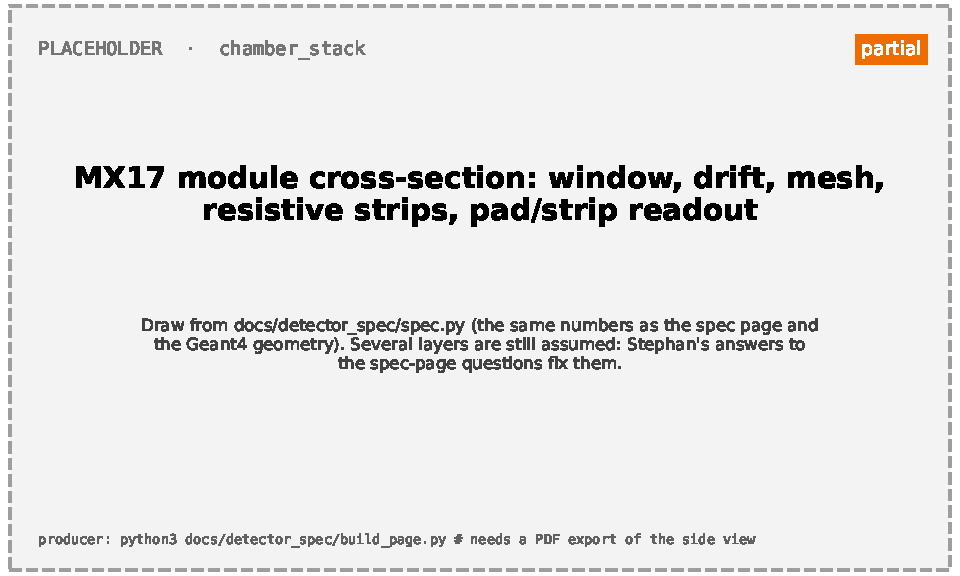
\includegraphics[width=0.9\linewidth]{chamber_stack}
  \caption{\tbw{Cross-section of the MX17 module, to scale in $z$ for the amplification region.}}
  \label{fig:stack}
\end{figure}
\begin{figure}[t]
  \centering
  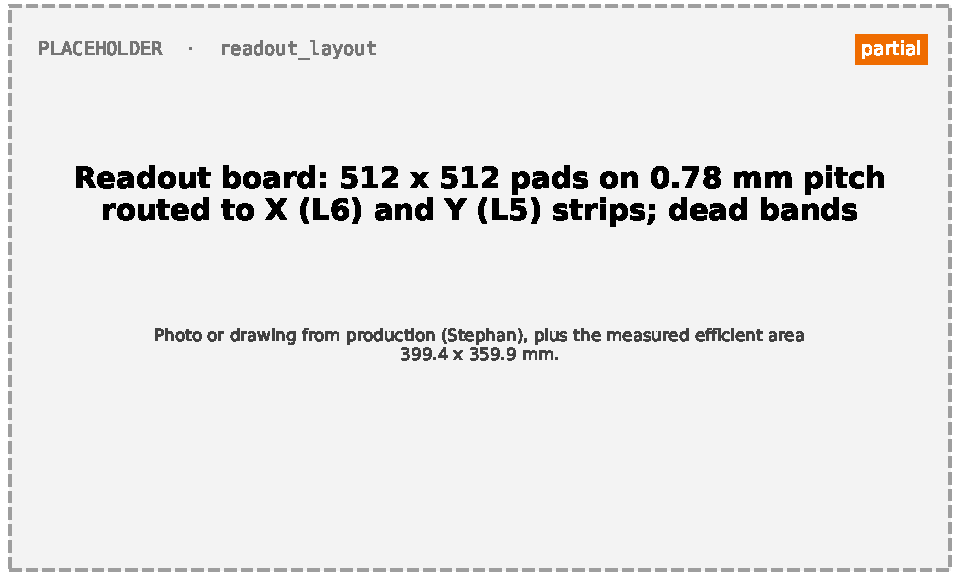
\includegraphics[width=0.8\linewidth]{readout_layout}
  \caption{\tbw{Readout board: pad pattern, X/Y routing and the dead bands.}}
  \label{fig:readout}
\end{figure}

\subsection{Production and quality control}
\tbw{How many boards were built, where and when; the bulk process; the resistive-layer printing; acceptance tests
(resistance mapping, HV training, leak and gas tightness, gain uniformity). Which board went into which chamber.}
\askStephan{This subsection is yours: production sequence, QA steps and their results, and anything that
distinguishes the boards of det2, det3, det4, det6 and det7 (in particular the det4 board, \cref{sec:det4}).}

\section{Test setups}\label{sec:setups}
\sectionstate{ready}{\texttt{mx\_june\_cosmic\_qa/MICROTPC\_RUNBOOK.md}; \texttt{sps\_beam\_test\_26/analysis/README.md}; \texttt{mpgd26} renders}
\intent{The two setups and what each can measure: the Saclay cosmic bench (M3 reference tracking, all five chambers,
June 2026) and the SPS H4 beam (uRWELL telescope, det4 only, including the 25.6\textdegree{} rotation).}

\subsection{Cosmic bench}
\tbw{Scintillator trigger, four M3 reference planes, two test slots. M3 recipe ($\chi^2<1.0$, $N_\mathrm{clus}=4$).
DREAM readout, sampling, window. Gas and flow.}
\askDylan{Gas per setup: bench Ar/iC$_4$H$_{10}$ 95/5? SPS runs with Ar/CF$_4$/iC$_4$H$_{10}$ 88/10/2? Which runs enter the paper?}

\begin{figure}[t]
  \centering
  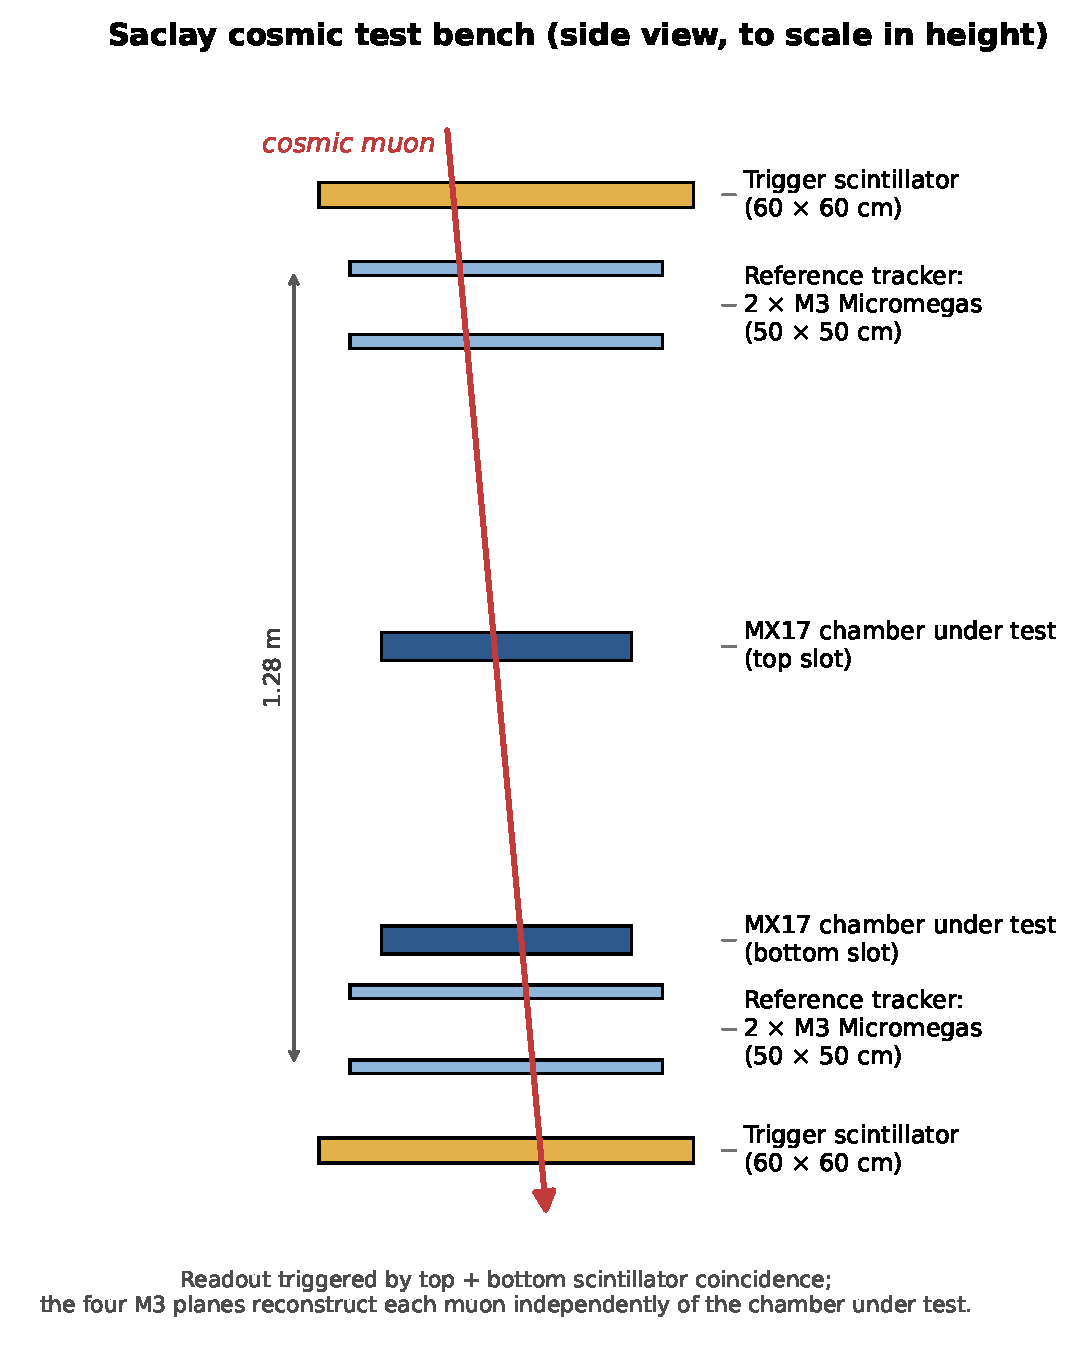
\includegraphics[width=0.75\linewidth]{bench_setup}
  \caption{The cosmic bench: scintillator trigger and four M3 reference planes around the two MX17 test slots.}
  \label{fig:bench}
\end{figure}

\subsection{SPS H4 beam}
\tbw{Beam, uRWELL references, det4 position, runs used (HV, drift field, gas, rotation).}
\begin{figure}[t]
  \centering
  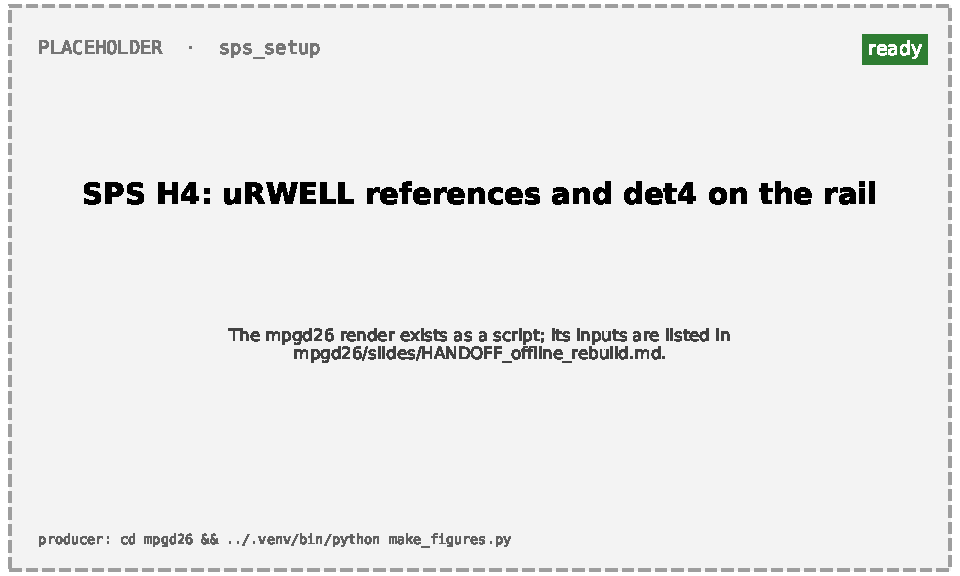
\includegraphics[width=0.85\linewidth]{sps_setup}
  \caption{\tbw{The SPS H4 setup.}}
  \label{fig:sps}
\end{figure}

\section{Operation: high voltage, gain and sparks}\label{sec:operation}
\sectionstate{ready}{topic 6 (HV scans, \texttt{10\_hv\_scan\_*.py}); PLAN\_39 (\texttt{39\_spark\_deadtime.py}); spark waveforms (\texttt{40\_spark\_waveforms.py}); \texttt{det3\_spark\_analysis}}
\intent{Where the chambers run and why: efficiency plateau against spark rate, the chosen operating points,
and the evidence that the resistive layer does its job (sparks stay local and cost no dead time).}

\tbw{Mesh-voltage scans per chamber; plateaus and the chosen points (480/480/440\,V). Spark rate Poisson,
muon-induced (4--6$\times$), concentrated at the edges; no post-spark dead time.}
\askStephan{Expected gain curve and spark behaviour for this resistivity: does what we see match production tests?}

\begin{figure}[t]
  \centering
  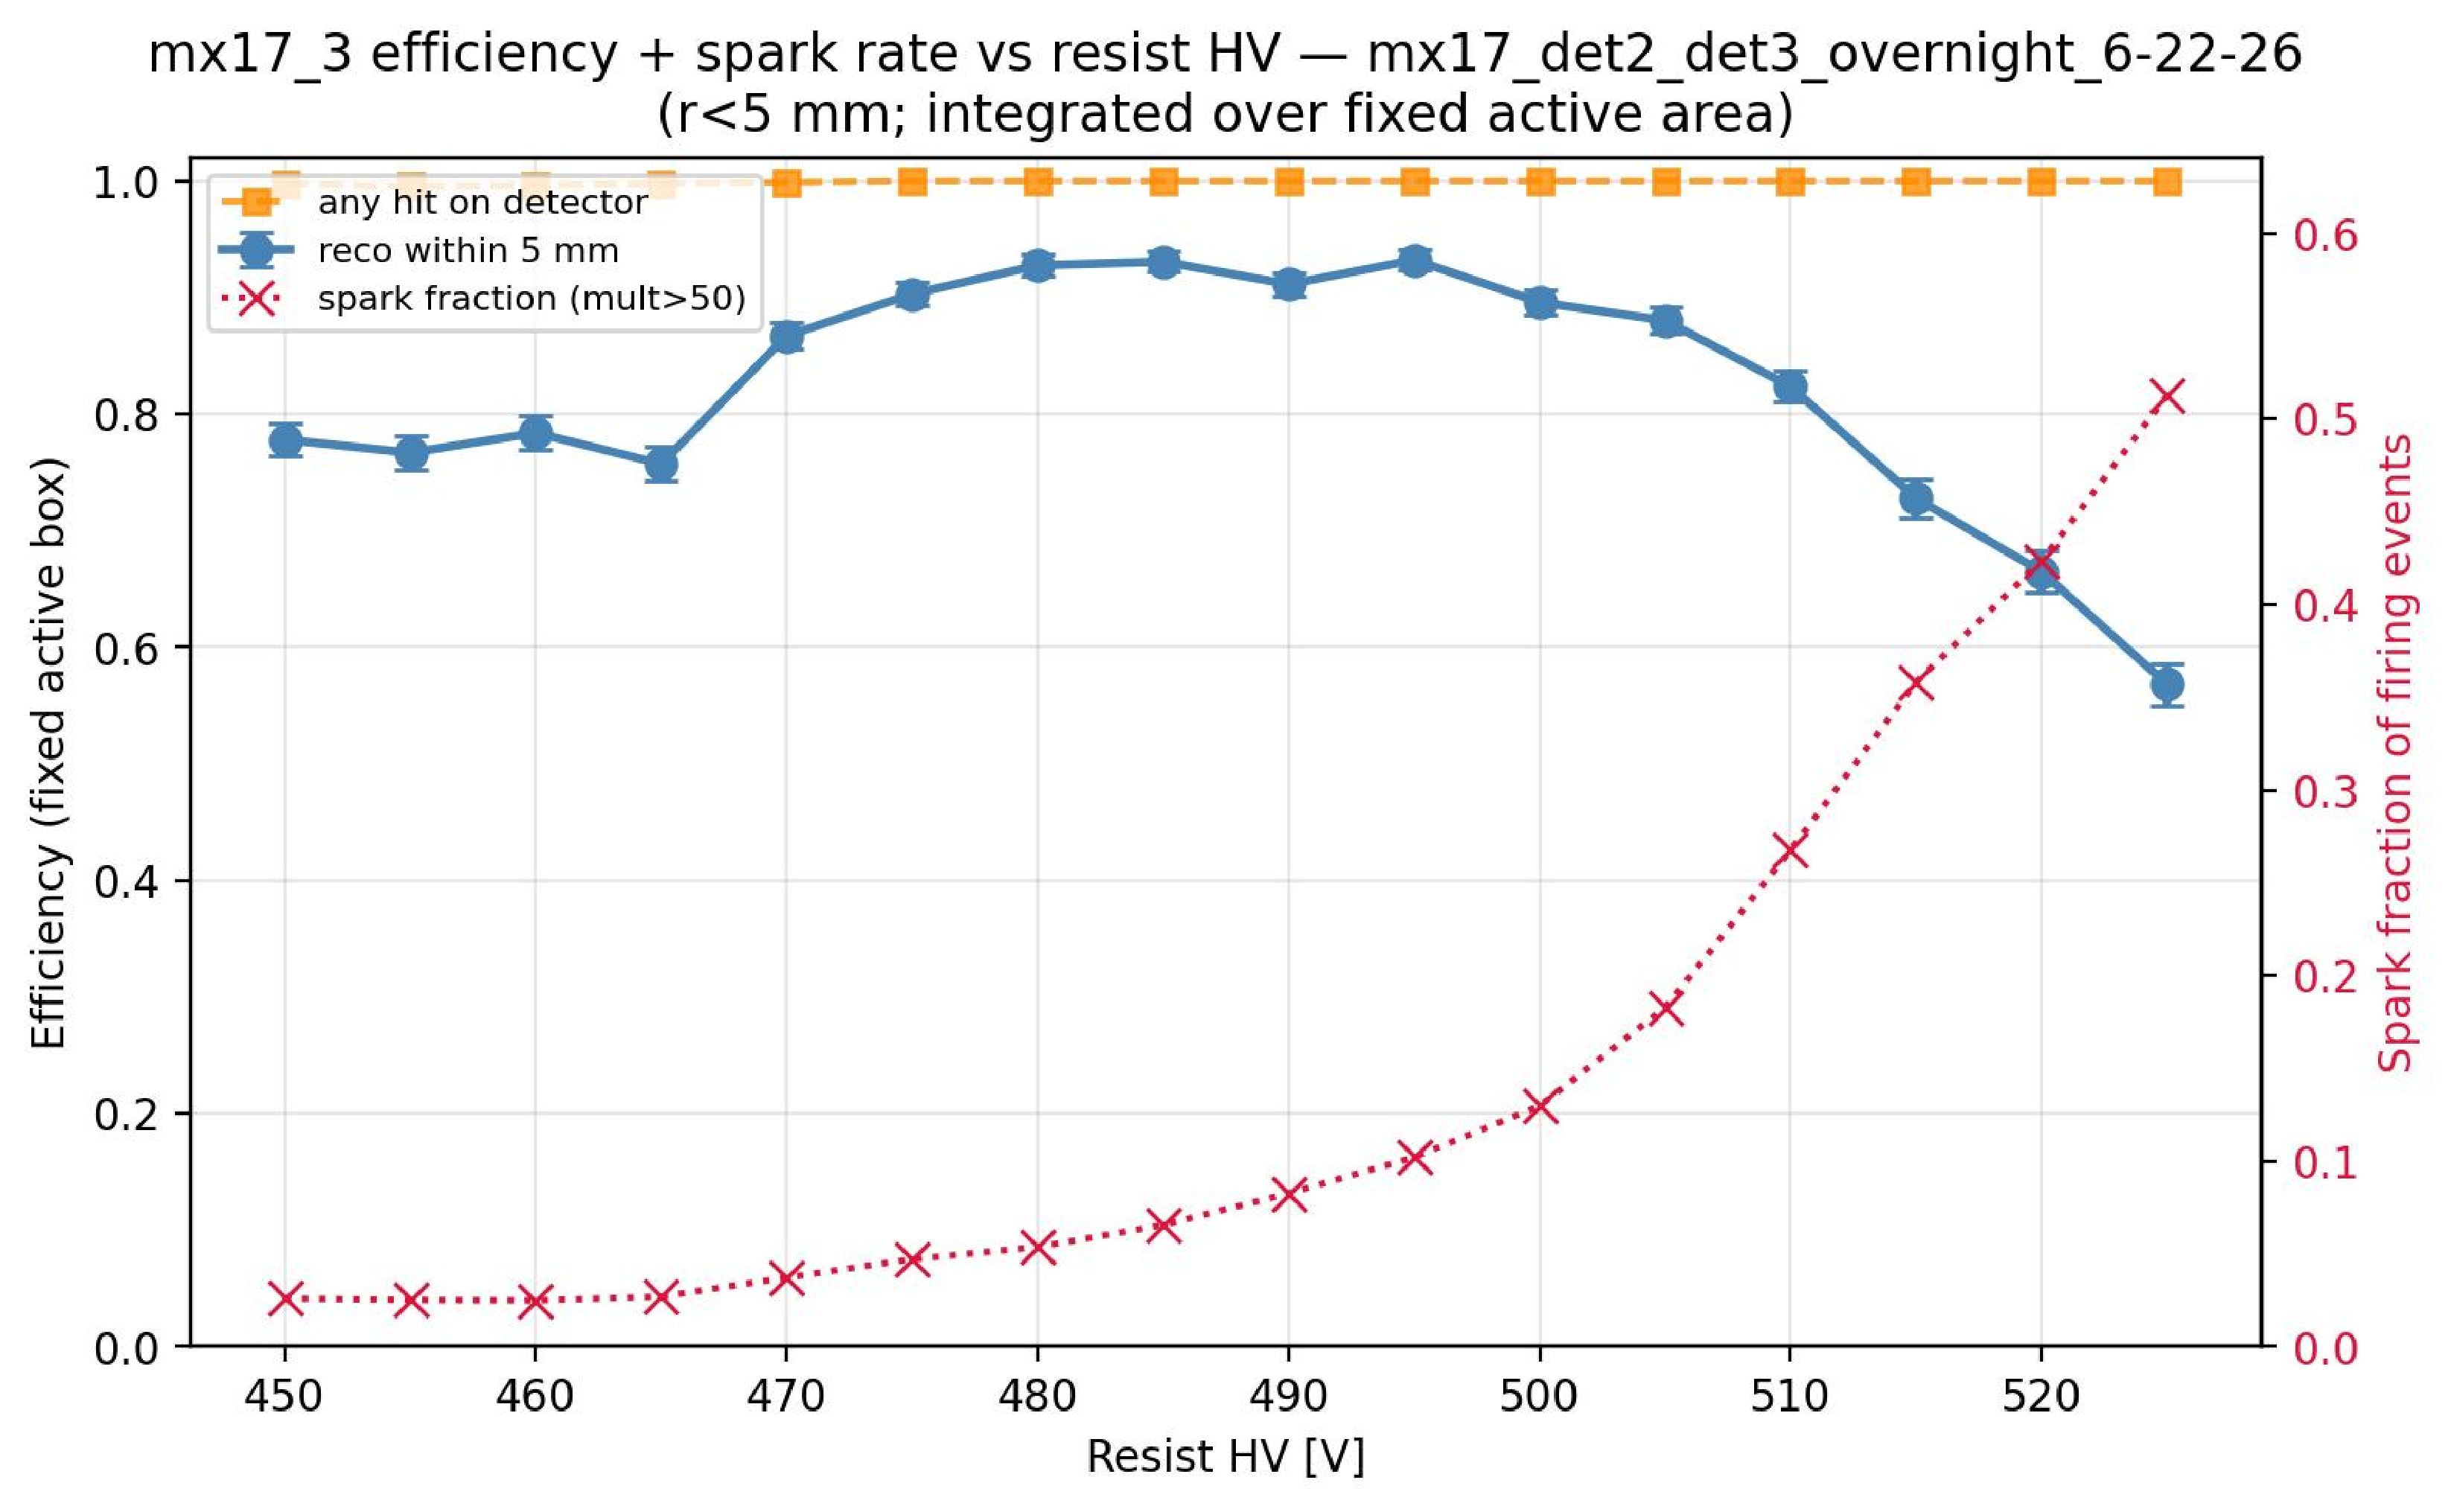
\includegraphics[width=0.75\linewidth]{hv_scan}
  \caption{\tbw{Mesh-voltage scan (det3): detection efficiency and spark rate.}}
  \label{fig:hv}
\end{figure}
\begin{figure}[t]
  \centering
  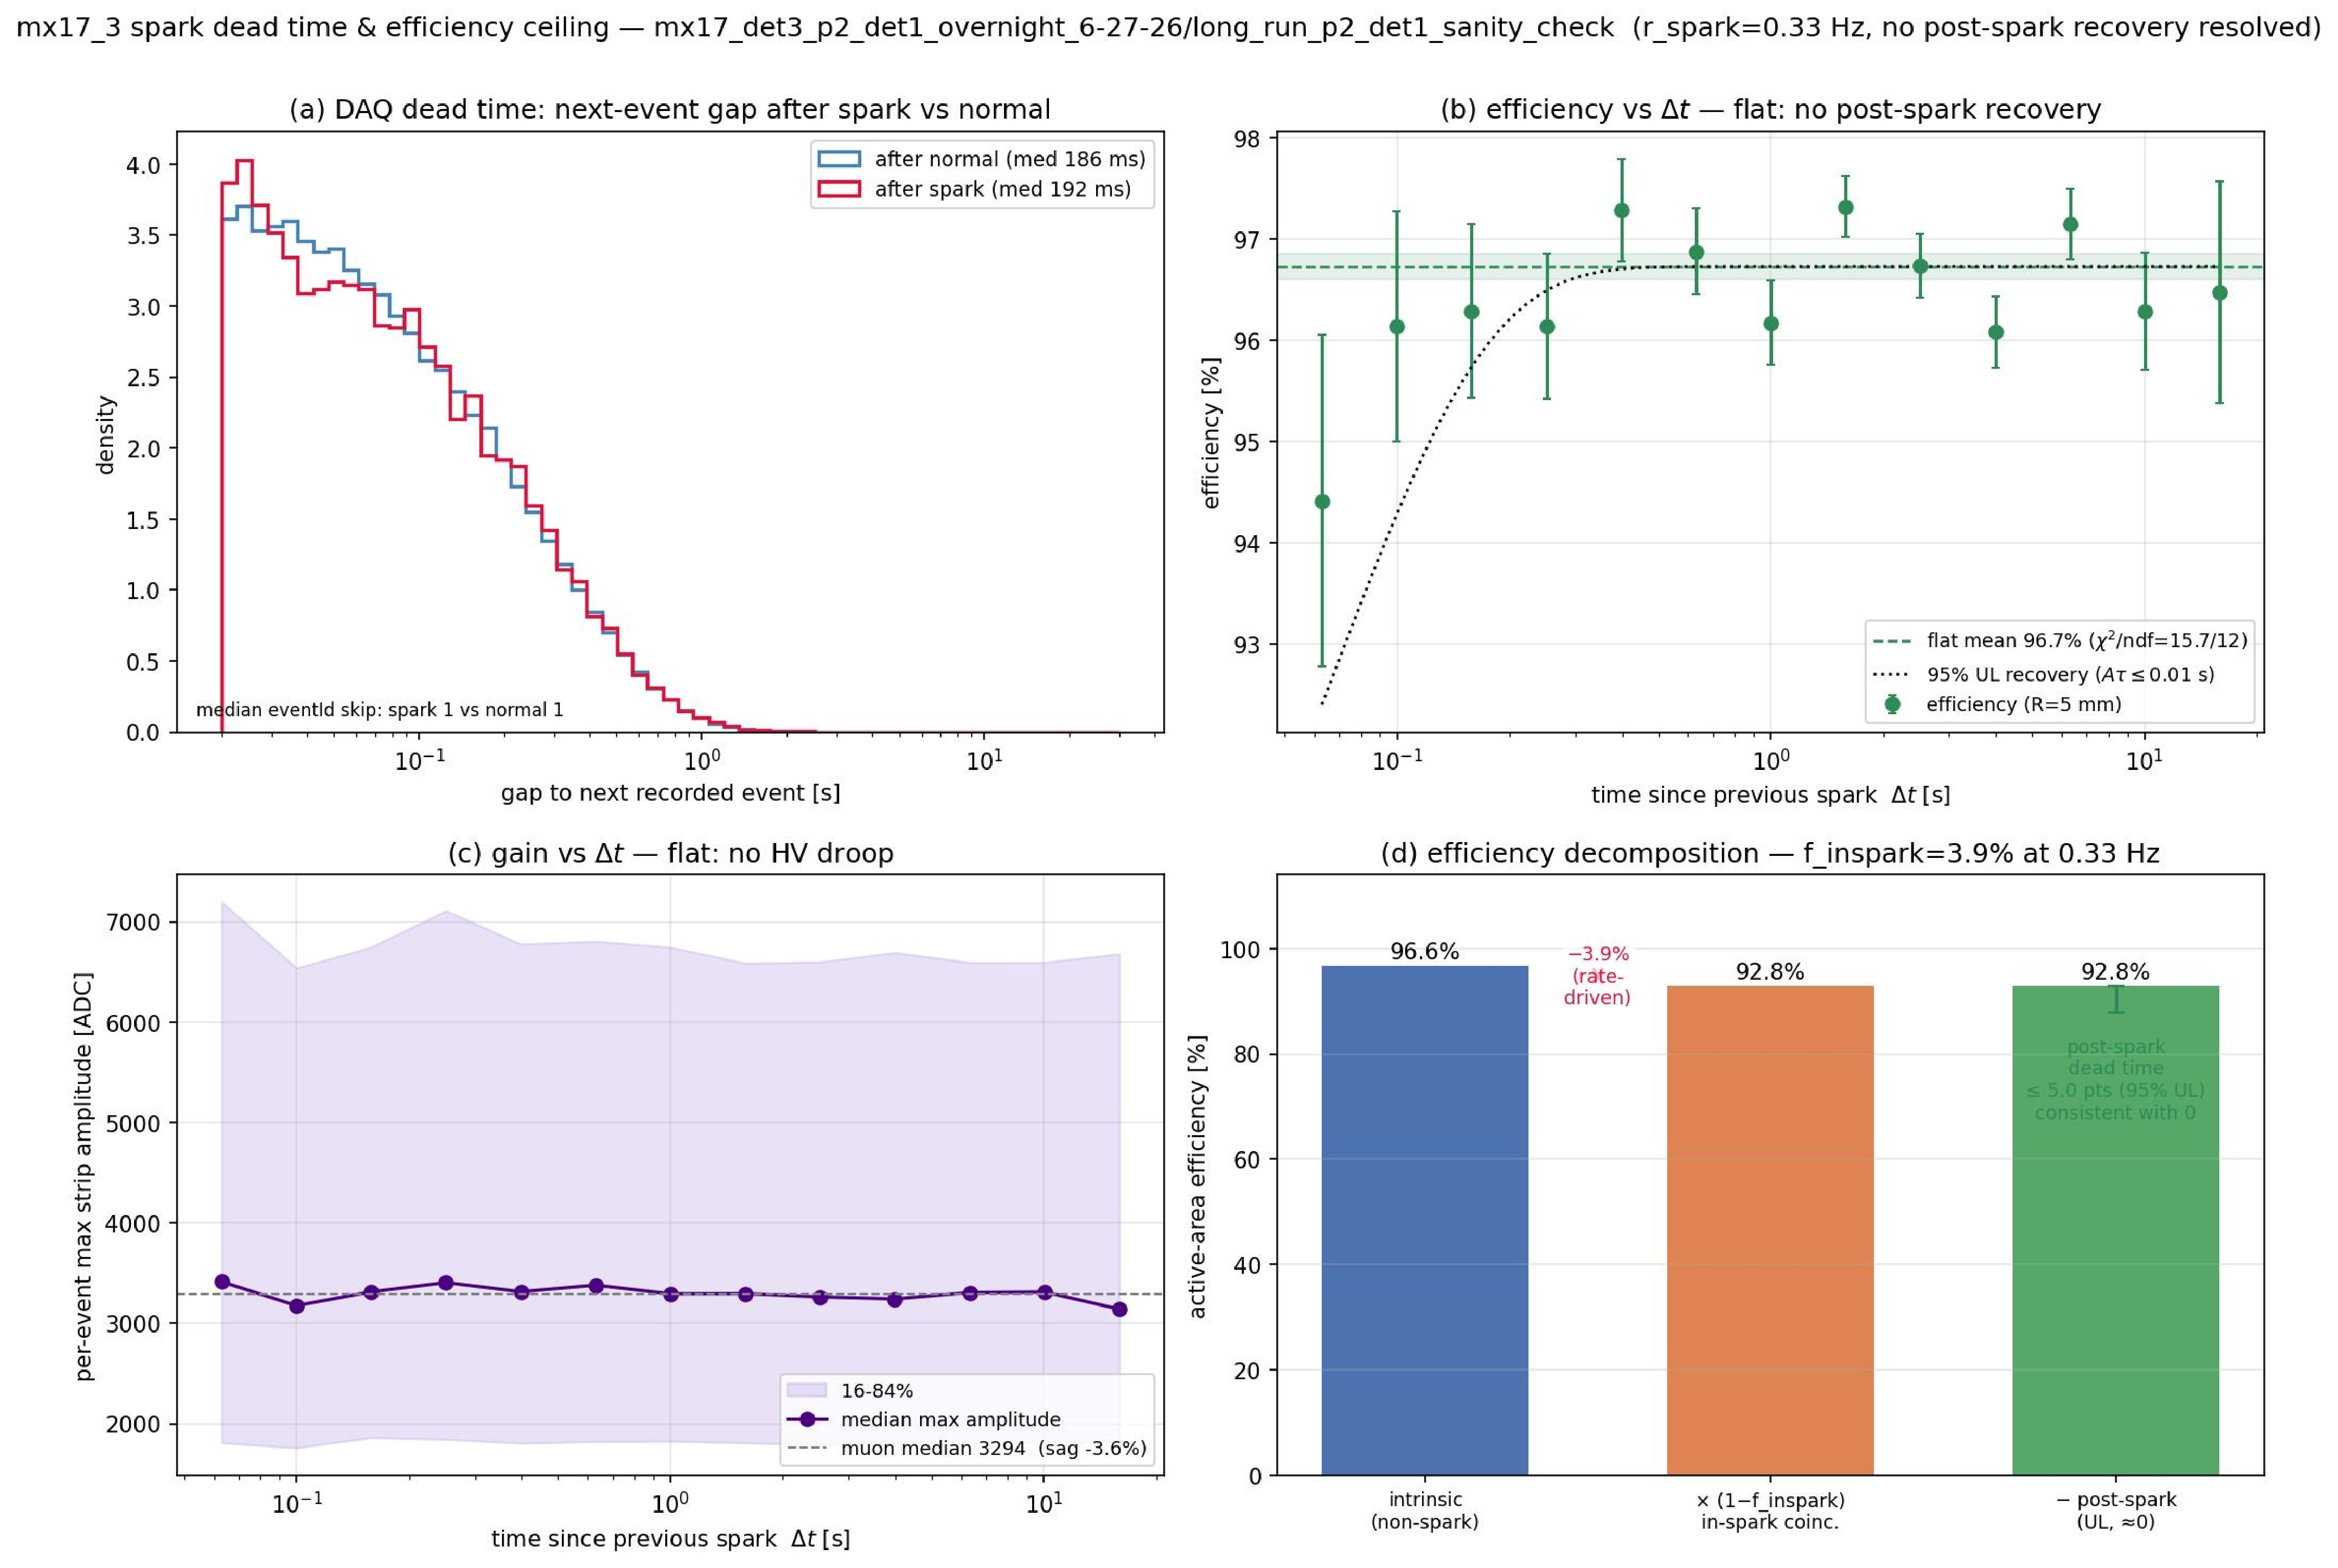
\includegraphics[width=0.75\linewidth]{spark_deadtime}
  \caption{\tbw{Efficiency in the time after a spark: no dead time.}}
  \label{fig:sparkdt}
\end{figure}

\section{Charge balance and efficiency}\label{sec:efficiency}
\sectionstate{partial}{PLAN\_38 (\texttt{38\_xy\_charge\_balance.py}); efficiency maps (\texttt{08}, \texttt{09}); edge study \texttt{32\_edge\_fringe\_field.py} (hits angle, D4)}
\intent{How the charge divides between the two views, and where each chamber is efficient. Hits are the right input
here (detection, amplitude); positions come from the M3 reference, not from the chamber.}

\subsection{X/Y charge balance}
\tbw{$f=q_X/(q_X+q_Y)$: median 0.487 (det3) and 0.531 (det2), $\sigma_{68}=0.07$, flat in position and angle; three charge proxies agree.}
\begin{figure}[t]
  \centering
  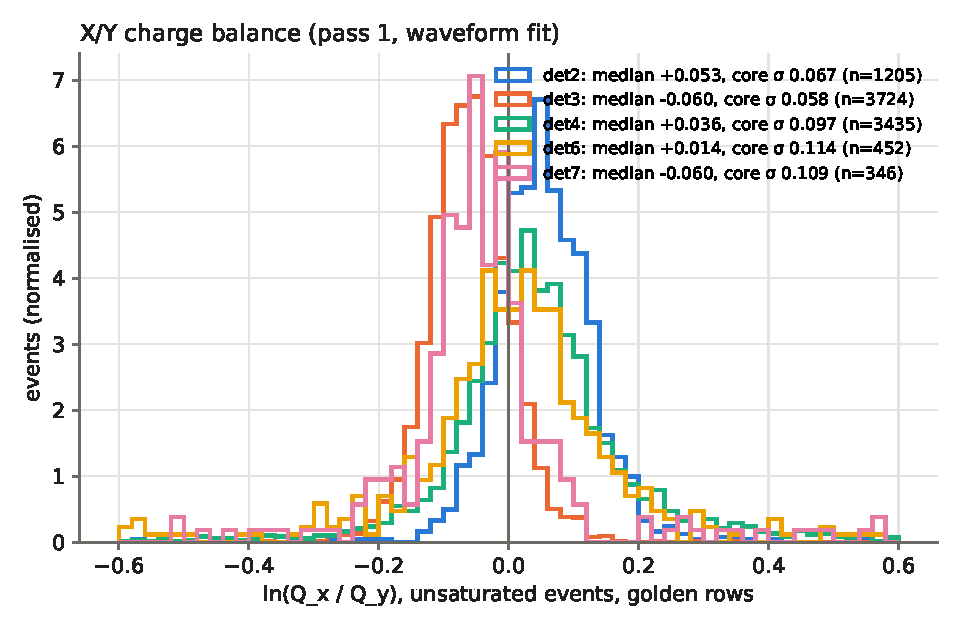
\includegraphics[width=0.6\linewidth]{charge_balance}
  \caption{\tbw{X/Y charge balance.}}
  \label{fig:balance}
\end{figure}

\subsection{Efficiency and maps}
\tbw{Detection efficiency per chamber; maps; the edge turn-on. Efficiency within 5\,mm:
\requote{93/92/42/75/57\,\%} (det3/2/4/6/7). det4's low value is its non-amplifying area (\cref{sec:det4}).}
\analysis{D1}{re-quote from the reproduced r06 products}
\analysis{D4}{edge angle tilt with wft angles}
\begin{figure}[t]
  \centering
  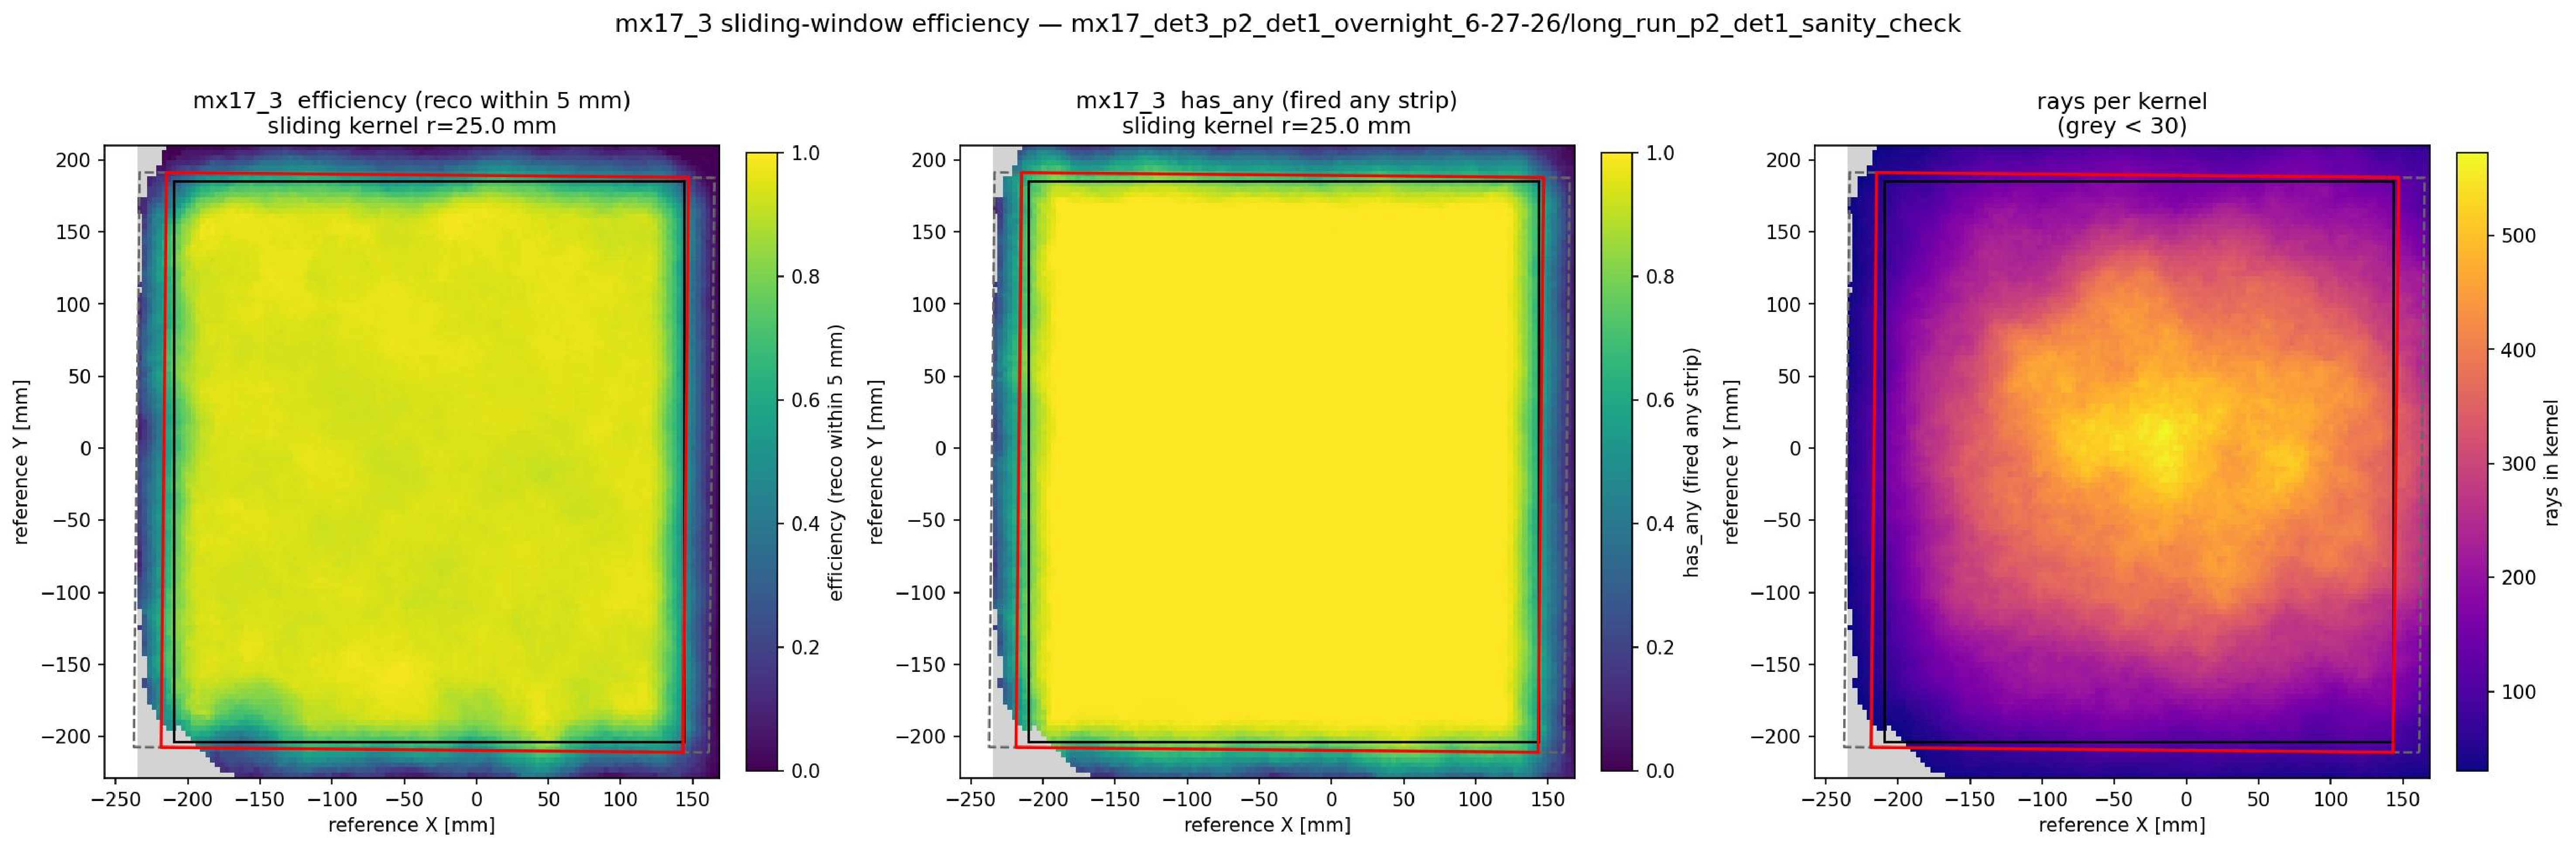
\includegraphics[width=0.7\linewidth]{efficiency_map}
  \caption{\tbw{Efficiency map (det3).}}
  \label{fig:effmap}
\end{figure}
\begin{figure}[t]
  \centering
  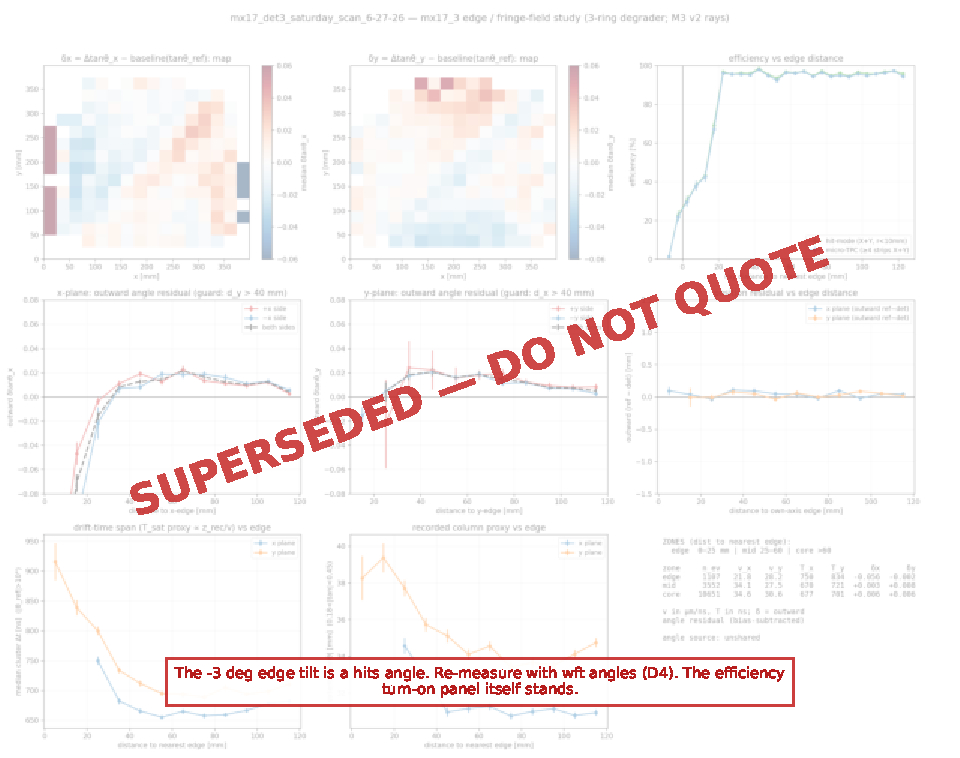
\includegraphics[width=0.7\linewidth]{edge_turnon}
  \caption{\tbw{Efficiency turn-on at the chamber edge.}}
  \label{fig:edge}
\end{figure}

\section{Gas: drift velocity and attachment}\label{sec:gas}
\sectionstate{partial}{\texttt{sps\_beam\_test\_26/analysis/cloud\_basics} \S16--27 (FINDINGS); notes \texttt{mx17-beam-attachment}, \texttt{mx17-sps-to-bench}}
\intent{The gas the chambers actually ran with, measured from the waveforms with one physics model and no free
loss rate: water sets the drift velocity, O$_2$ sets the attachment.}

\tbw{Bench (det3 drift scan, six fields 35--382\,V/cm): $v$ = 2.5--37.8\,\textmu m/ns, 0.95\,\% water, no air
($\lesssim$10\,ppm O$_2$). Beam run\_71: 1.51\,\% water and 163\,ppm O$_2$, attachment measured in X and Y;
run\_63 230$\to$147\,ppm overnight. The beam O$_2$ does not spoil the SPS readout constants. Gap topography
(bench det3 spread 1.5\,mm). Magboltz~\cite{Biagi1999}.}
\analysis{D2}{v(E) points reconstructed on r06}
\analysis{D5}{three-body O$_2$ attachment scale (ppm is model-dependent)}
\askStephan{Gas system on the bench: flow, materials, expected outgassing / water ingress?}

\begin{figure}[t]
  \centering
  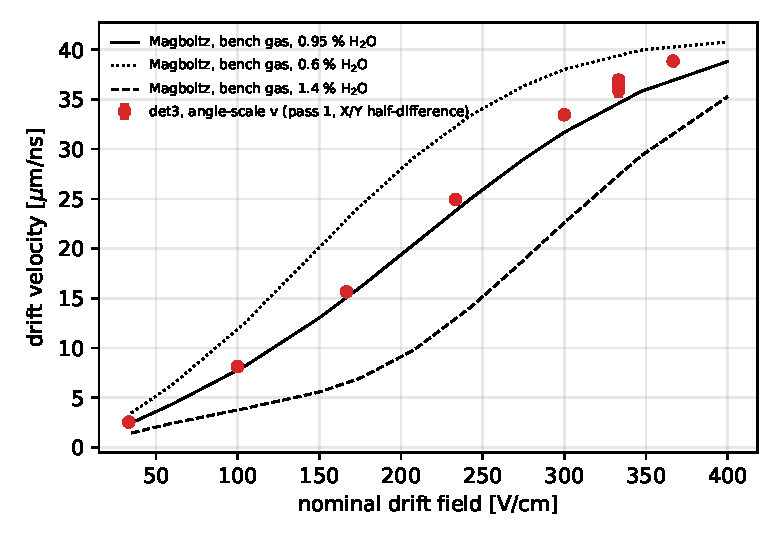
\includegraphics[width=0.7\linewidth]{gas_vE}
  \caption{\tbw{Drift velocity against field, waveform fit and Magboltz.}}
  \label{fig:vE}
\end{figure}
\begin{figure}[t]
  \centering
  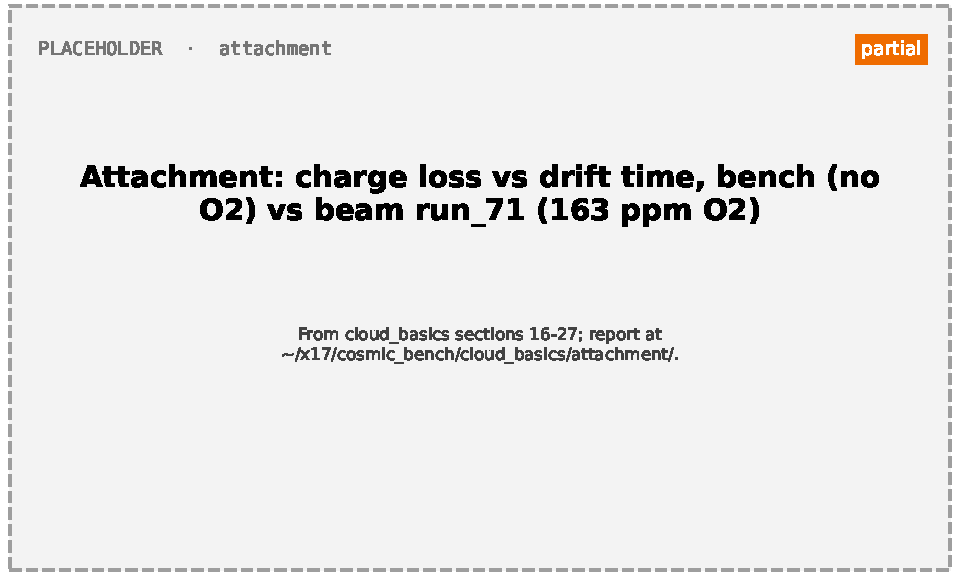
\includegraphics[width=0.7\linewidth]{attachment}
  \caption{\tbw{Charge loss with drift time: bench and beam.}}
  \label{fig:attach}
\end{figure}

\section{Timing}\label{sec:timing}
\sectionstate{open}{PLAN\_42 (\texttt{42\_time\_resolution.py}) -- hits-based; waveform port is D3}
\intent{The time resolution of a chamber against the scintillator trigger, which fixes how well the absolute drift
depth (and so the $z$ of a track) is known.}

\tbw{Method: scintillator-trigger reference, DREAM fine timestamp. The hits value (33\,ns) is not quoted; waveform result to come.}
\analysis{D3}{time resolution on waveforms}
\begin{figure}[t]
  \centering
  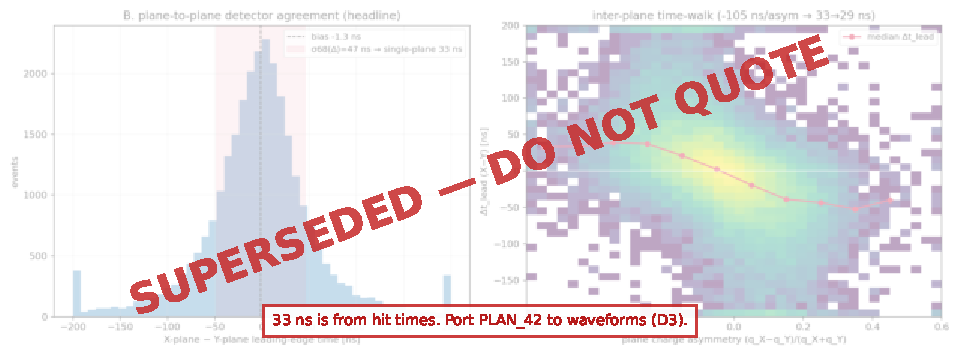
\includegraphics[width=0.7\linewidth]{timing}
  \caption{\tbw{Time resolution.}}
  \label{fig:timing}
\end{figure}

\section{Tracking performance and resolution}\label{sec:tracking}
\sectionstate{requote}{\texttt{mx\_june\_wft/FLEET\_DIGEST.md} (r06, reproduced 10-09, C1); \texttt{sps\_beam\_test\_26/analysis/spatial\_resolution}}
\intent{What the chambers deliver with the reconstruction of the companion paper~\cite{paperII}: angle and position
on cosmics for all five chambers, and the intrinsic resolution of det4 in the beam with the reference fitted out.}

\subsection{Cosmic rays}
\tbw{$\sigma_\theta$ = \requote{1.15--2.51\textdegree}, better than hits on every plane; position residuals; bias; per chamber.}
\analysis{D1}{re-quote from r06}
\askDylan{C2: freeze r06 as it is, or the per-plane c2/c1 (pvy95 re-pass, staged)?}
\begin{figure}[t]
  \centering
  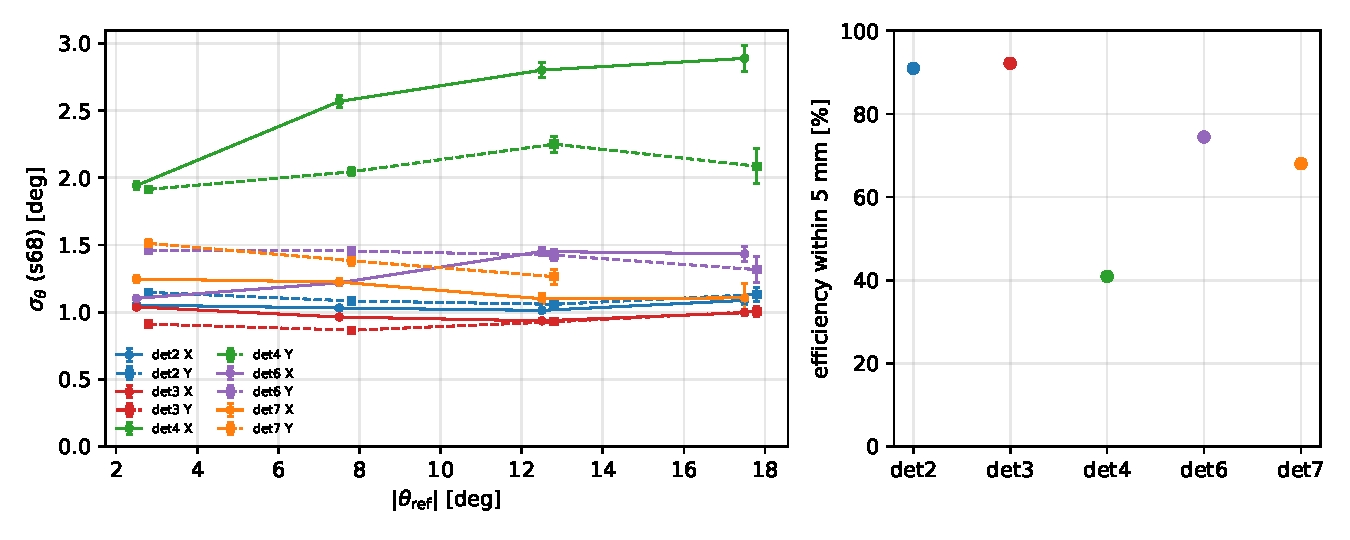
\includegraphics[width=0.85\linewidth]{tracking_perf}
  \caption{\tbw{Cosmic tracking performance, five chambers.}}
  \label{fig:trackperf}
\end{figure}

\subsection{Intrinsic resolution in the beam}
\tbw{det4 at SPS: $176\pm10$\,\textmu m $=0.30\times$ pitch, reference fitted out. The bench 0.6--0.7\,mm is
M3 pointing $\oplus$ $\sim$1.1\,mrad multiple scattering (arithmetic).}
\analysis{D6}{optional: bench resolution decomposed by measurement or simulation}
\begin{figure}[t]
  \centering
  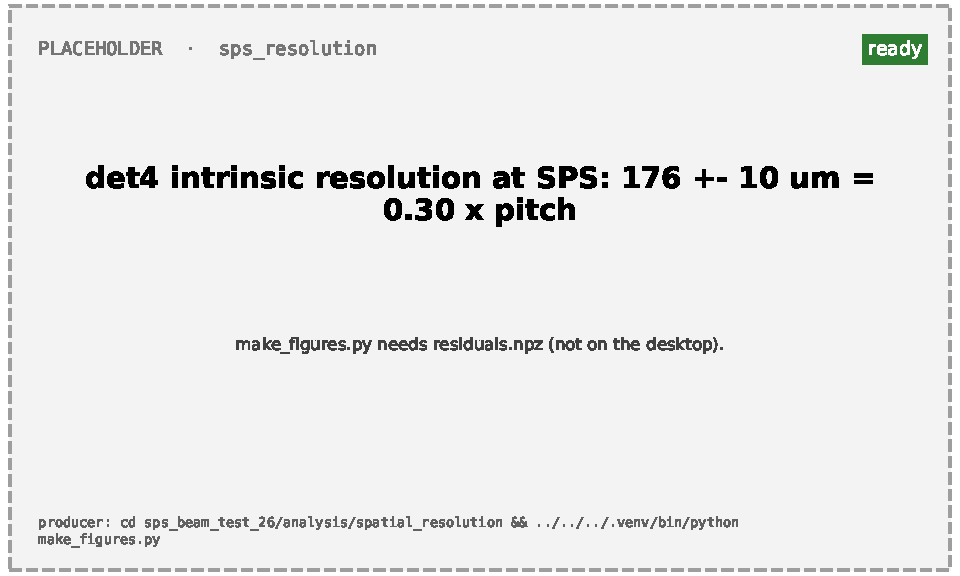
\includegraphics[width=0.7\linewidth]{sps_resolution}
  \caption{\tbw{det4 residual decomposition in the SPS beam.}}
  \label{fig:spsres}
\end{figure}

\subsection{The readout plane is not flat: a bow of the readout boards}\label{sec:bow}
\sectionstate{partial}{model-audit follow-up FB, \texttt{rerun/model\_audit/followups/fb\_bow\_maps/} (2026-10-27); slide note \texttt{notes/mx17-chamber-bow}}
\intent{Establish, from bench data alone, that the mesh surface of every chamber is dished by 1--3\,mm and that the drift
direction follows its slope; give its size per chamber, its sign from external facts, how stable it is, the evidence
that excludes the alternatives, and what correcting for it gains. Draft (2026-10-27).}

A micro-TPC converts the time structure of the induced signals into a track angle under two assumptions about the
chamber: that the readout plane is flat and that the drift field is perpendicular to it. On all five chambers measured on
the cosmic bench, both assumptions fail at the millimetre level, in the way a bowed readout board predicts.

\paragraph{Three independent observables.}
(i)~\emph{Positions.} A track of slope $\tan\theta = \mathrm{d}x/\mathrm{d}z$ crosses a mesh displaced by $h$ along $z$
at a point shifted by $h\tan\theta$. In every position cell the slope of the position residual (fitted mesh position
minus the M3 prediction) against the M3 slope is therefore the local mesh height $h(x,y)$. It is measured independently
by the X and the Y strips, through the two independent M3 projections. Both views see a dish in both directions
(Fig.~\ref{fig:bowprof}): the centre lies $1.5$--$2.3$\,mm below a point 150\,mm out along either axis
(det2 $1.8\pm0.2$, det3 $1.5\pm0.2$, det4 $1.9\pm0.2$, det6 $1.8\pm0.2$, det7 $2.3\pm0.4$\,mm), i.e.\ a curvature of
$1.3$--$2.1\times10^{-4}$\,mm$^{-1}$.
(ii)~\emph{Drift tilt.} If drift lines leave the mesh normal to its surface, charge produced at height $d$ arrives
displaced by $d\,\partial h/\partial x$, so the fitted transverse speed acquires an offset
$w_0 = v\,r_f\,\partial h/\partial x$ with $r_f$ between $1/2$ (flat cathode) and 1 (cathode bowed with the board).
For a dish, $w_0$ must rise linearly across the chamber. It does, in all ten chamber views, by
$\pm0.6$\,\textmu m/ns over 300\,mm, with $r_f = 0.4$--$0.9$ on nine of ten views (Fig.~\ref{fig:bowclos}). The
sign of this relation is predicted by the geometry, not fitted.
(iii)~\emph{Narrowest cluster.} The cluster of strips above threshold is narrowest for the track running along the
local drift lines, at $\tan\theta = -w_0/v$. This uses amplitudes only, with no hit times and no fitted angle; the
narrowest-cluster slope drifts across the chamber with the predicted sign on 9/10 views.

\paragraph{Sign.}
The M3 $z$ axis points up (the ray files carry the top and bottom M3 plane heights, 1302 and 24\,mm; the upper DUT slot
is at 702\,mm, the lower at 232\,mm), and the chambers lie with the readout board down and the cathode up (the fitted
micro-TPC slope has the sign of the M3 slope on every chamber). The mesh centre is therefore \emph{lower} than its rim,
further from the cathode: the direction in which the board's weight, gas overpressure and residual mesh tension all push.

\paragraph{Alternatives.}
A plane-scale error of the telescope that could produce the $w_0$ ramp would leave a $\sim$6\,\% position scale at the
chamber; the measured residual scale is below 0.15\,\%. A position-dependent $t_0$ bias would vanish when every track is
moved to a fixed trigger latency; 80--100\,\% of the curvature survives. Fringe fields at the frame decay within
$\sim$10\,mm of the edges, while the ramp is linear over 300\,mm. A bow of the M3 planes would shift tracks by
$\tan\theta\, g(x,y)$ and can mimic $h$, but cannot produce $w_0$ or move the narrowest cluster; a common telescope
contribution to the depth cannot be excluded and limits the depth to $0.5$--$1.3$ times the quoted value.
The column duration, which should lengthen where the gap deepens, does not resolve the effect: its X and Y readings of
the same column differ by more than the 1--2\,mm expected.

\paragraph{Stability.}
Nineteen bench runs were reconstructed with each chamber's own calibration and their own alignment: other subruns of
the same night, other nights (det2 after a remount, det3 and det4 on other days), both bench slots (det3 at $z=702$ and
$232$\,mm) and other drift and mesh voltages. Fifteen give their chamber's dish depth within $2\sigma$; the one clear
outlier is det3 on 6-25 ($0.9\pm0.1$\,mm against a det3 mean of $\approx1.5$\,mm), while det3 in the same lower slot on
6-23 reads $1.7\pm0.1$\,mm. The drift-tilt shape measured on one run, applied to the others with only the rigid tilt
re-measured, recovers a median 94\,\% of the angular-resolution gain of each run's own map. The bow is therefore a
static property of each chamber at the 20\,\% level; which load sets it cannot be separated with the data available.

\paragraph{Plausibility.}
The 1.7\,mm readout PCB spans the 0.40\,m aperture of its support plate with only 5\,mm of Rohacell behind it. A
Kirchhoff-plate estimate gives a dip at 150\,mm of 0.1--0.25\,mm from its own weight, 0.3--0.7\,mm per mbar of gas
overpressure and up to $\sim$1\,mm from a mesh laminated under 10\,N/cm: the measured depth needs no exotic load.

\paragraph{Correction.}
The bow enters the reconstruction only through the conversion of the fitted transverse speed into an angle and through
the height of the track point. A per-chamber surface (static shape) plus the per-run rigid tilt, validated by two-fold
cross-validation on held-out tracks, improves the angular resolution by a median of 16\,\% (1--30\,\% per view); the
shape predicted from positions alone, with two numbers fitted to the angles, recovers 15\,\%. With the final reconstruction settings (one prompt footprint $\sigma_0=0.30$\,mm for both views, pinned $t_0$, 20\,ns grid) the same map still improves the Y-view resolution by 13--25\,\% and removes a $-8$\,\% steep-track compression on det6\,X. Subtracting
$h\tan\theta$ improves the position residual by 4--15\,\%. Because the load depends on mounting and the chambers
stand vertical at n\_TOF, the bench surface is not transferred to the beam data without an in-situ measurement.
\askDylan{Is a direct flatness measurement of a spare board (or the photographs of the opened chambers) available to
quote alongside? No new data are needed for the text as it stands.}

\begin{figure}[t]
  \centering
  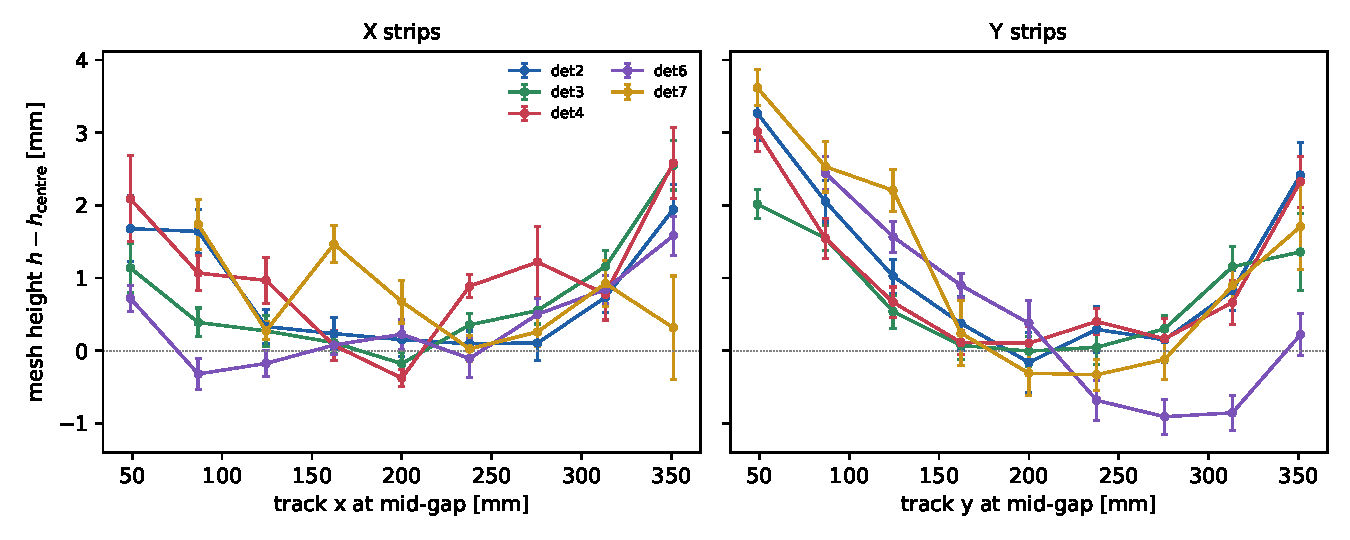
\includegraphics[width=0.95\linewidth]{bow_profiles}
  \caption{Mesh height across the chamber from position residuals against the M3 track slope, for the X (left) and Y
  (right) strips of the five chambers, relative to the fitted parabola's value at the centre. Golden bench rows.}
  \label{fig:bowprof}
\end{figure}
\begin{figure}[t]
  \centering
  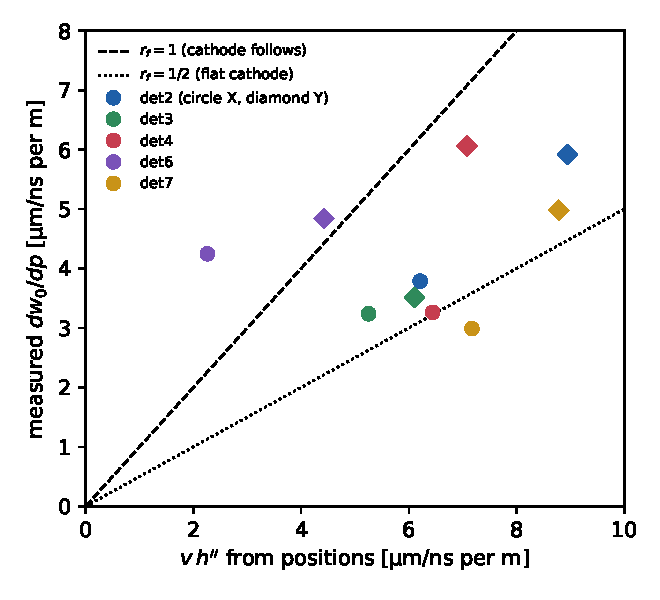
\includegraphics[width=0.5\linewidth]{bow_closure}
  \caption{Gradient of the drift-tilt offset $w_0$ across the chamber against the gradient predicted from the
  position-route curvature, $v\,h''$. Lines: drift lines tilted fully with the mesh ($r_f=1$) and a flat cathode
  ($r_f=1/2$). Circles X strips, diamonds Y strips.}
  \label{fig:bowclos}
\end{figure}

\section{det4: the non-amplifying stripes}\label{sec:det4}
\sectionstate{ready}{\texttt{sps\_beam\_test\_26/det4\_sps\_assessment} (scripts 01--17)}
\intent{A production defect seen in the data: 62\,\% of det4's area does not amplify, in stripes. What the data say
about its cause, and why det4's bench numbers are low.}

\tbw{Board map, periodicity, connector and strip-break tests, HV headroom, stability across runs.}
\askStephan{Do the stripes match anything in det4's production (resistive printing, lamination, a particular step)?
Was it seen in QA? Is this paper the place to show it?}
\begin{figure}[t]
  \centering
  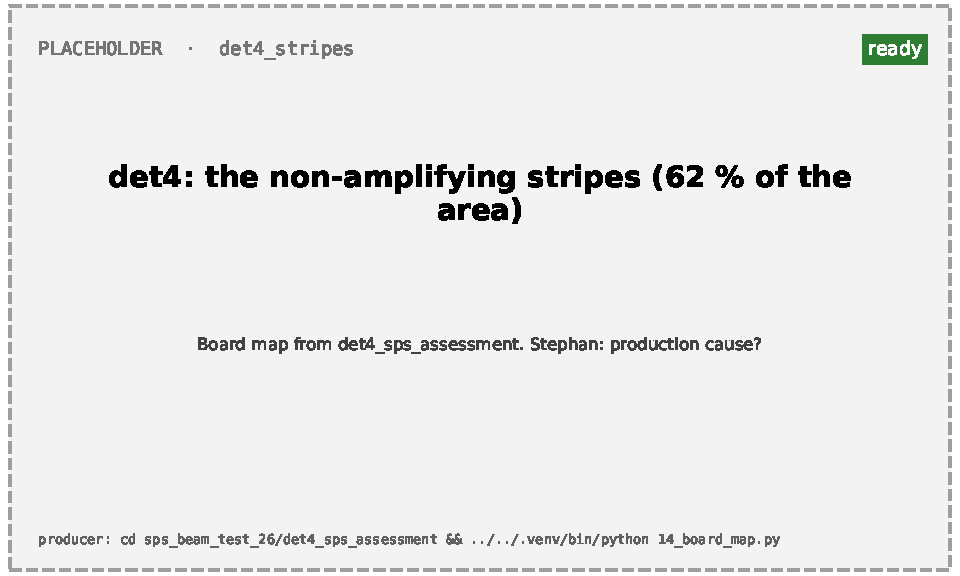
\includegraphics[width=0.75\linewidth]{det4_stripes}
  \caption{\tbw{det4 board map: amplifying and non-amplifying regions.}}
  \label{fig:det4}
\end{figure}

\section{Conclusions}\label{sec:conclusions}
\sectionstate{open}{all of the above}
\tbw{What the chambers do, what limits them, what the n\_TOF campaign used them for.}


\appendix
\section{Where the inefficiency goes: loss categories}\label{app:losses}
\sectionstate{partial}{\texttt{rerun/effbudget} (ladder) + \texttt{rerun/outliers/classify.py} (classes) + \texttt{rerun/satstudy} (displays, recovery tests); note \texttt{notes/mx17-det3-loss-categories}. Numbers are on the pre-pass golden table: re-derive on the re-processing pass}
\intent{Every M3 track crossing the det3 interior that is not detected, followed to the one place it ends up: one real
event display per class, the fraction of tracks lost to it, its mechanism, and whether a reference-free change to the
reconstruction recovers it (tested by re-running the reconstruction, not argued). Dylan 2026-10-26: a full appendix.}

\begin{table}[h]
  \centering\small
  \caption{\tbw{det3 interior, \requote{6\,451} M3 tracks, \requote{91.2\,\%} detected within 5\,mm. First matching class wins.}}
  \label{tab:losses}
  \begin{tabular}{lrl}
    \hline
    class & lost [\%] & recoverable without the reference? \\
    \hline
    found, removed by the competing-cluster cut & \requote{2.11} & yes: choice of cut \\
    second particle (fit took another real track) & \requote{1.89} & no: M3 among candidates in 64\,\%, needs the reference to choose \\
    ``spark'': discharge & \requote{0.50} & no \\
    ``spark'': muon + unrelated deposit & \requote{0.76} & partly: veto off + cut relaxed, 19/49 \\
    ``spark'': shower at the crossing & \requote{0.70} & no \\
    $\delta$-ray on the track & \requote{0.93} & not with a straight-line model \\
    saturated $\delta$ blob, fit off & \requote{0.81} & not by censoring ($\le$2\,pts); needs a track\,+\,blob model \\
    two close tracks, fit between & \requote{0.34} & no (below the two-track limit) \\
    2-strip seed under the 10\,\% floor (``fit failed'') & \requote{0.26} & yes: \texttt{MIN\_STRIPS}\,=\,2, 17/17 \\
    edge of the other coordinate & \requote{0.29} & no (geometry) \\
    position tail ($\approx\frac23$ bent M3 tracks) & \requote{0.22} & no (reference) \\
    \hline
  \end{tabular}
\end{table}

\tbw{One paragraph and one event display per class (strip position $\times$ drift time, M3 line and fit drawn), from
\texttt{rerun/satstudy/make\_deck.py}'s \texttt{evd()}; figure ids \texttt{loss\_<class>} to be added to
\texttt{figures.toml}.}
\analysis{A1}{appendix figures: one display per class as PDF via figures.toml; re-derive the fractions on the pass tables; decide whether det2/det4/det6/det7 get a column}


\bibliographystyle{unsrt}
\bibliography{refs}
\end{document}
